\documentclass{standalone}
\usepackage{tikz}
\usetikzlibrary{shapes, arrows.meta, positioning}

\begin{document}

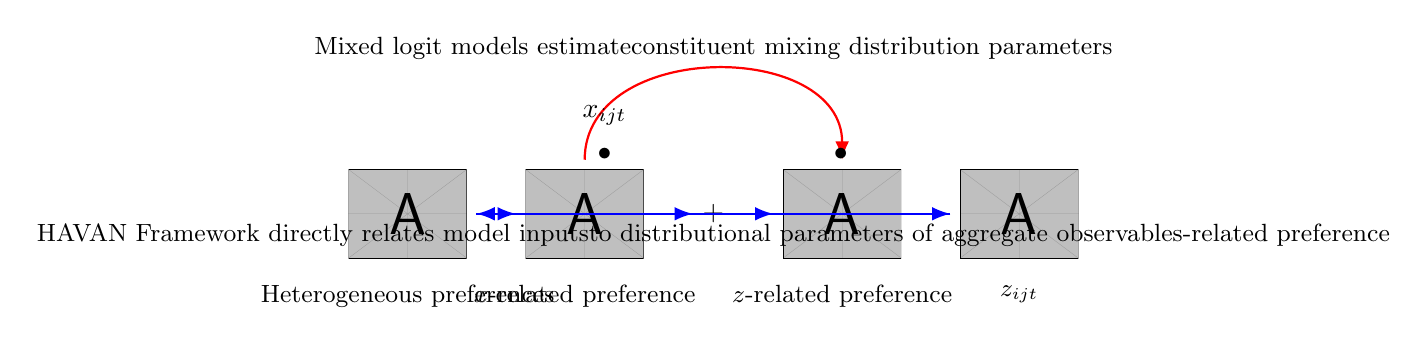
\begin{tikzpicture}
    % Styles
    \tikzstyle{arrow} = [blue, thick, -Latex]
    
    % Nodes
    \node (pref) at (0,0) {\includegraphics[width=1.5cm]{example-image-a}}; % Placeholder for Heterogeneous preferences image
    \node[right=0.5cm of pref] (xrel) {\includegraphics[width=1.5cm]{example-image-a}}; % Placeholder for x-related preference image
    \node[right=0.5cm of xrel] (plus) {+};
    \node[right=0.5cm of plus] (zrel) {\includegraphics[width=1.5cm]{example-image-a}}; % Placeholder for z-related preference image
    \node[right=0.5cm of zrel] (agg) {\includegraphics[width=1.5cm]{example-image-a}}; % Placeholder for Aggregate preferences image

    % Text labels
    \node[below=0.1cm of pref] {\small Heterogeneous preferences};
    \node[below=0.1cm of xrel] {\small $x$-related preference};
    \node[below=0.1cm of zrel] {\small $z$-related preference};
    \node[below=0.1cm of agg] {\small $z_{ijt}$};
    
    % Arrows
    \draw[arrow] (pref) -- (xrel);
    \draw[arrow, red] (xrel.north) to[out=90, in=90, looseness=1.2] node[above, black] {\small Mixed logit models estimate \\ \small constituent mixing distribution parameters} (zrel.north);
    \draw[arrow] (xrel) -- (plus);
    \draw[arrow] (plus) -- (zrel);
    \draw[arrow] (zrel) -- (agg);
    \draw[arrow, blue] (agg) to[out=180, in=0, looseness=1] node[below, black] {\small HAVAN Framework directly relates model inputs \\ \small to distributional parameters of aggregate observables-related preference} (pref);
    
    % Additional labels for equations
    \node at (2.5, 0.75) {$\bullet$};
    \node at (2.5, 1.25) {$x_{ijt}$};
    \node at (5.5, 0.75) {$\bullet$};
\end{tikzpicture}

\end{document}